\newpage
\section{Linear models}
\subsection{Regression}
\begin{definition}[Regressione]
	La regressione è il processo di stimare una funzione a numeri reali sulla base di un numero finito di esempi con un certo rumore.
\end{definition}
\begin{example}
	A partire dai seguenti valori
	\begin{table}[!h]
		\centering
		\begin{tabular}{|c|c|c|c|c|c|c|}
			\hline
			\textbf{Target} & $2.1$ & $3.9$ & $6.1$ & $8.4$ & $9.8$ & $\ldots$\\
			\hline
			\textbf{x} & $1$ & $2$ & $3$ & $4$ & $5$ & $\ldots$\\
			\hline
		\end{tabular}
	\end{table}
	trovare la funzione $f$ che li approssimi.
	\begin{center}
		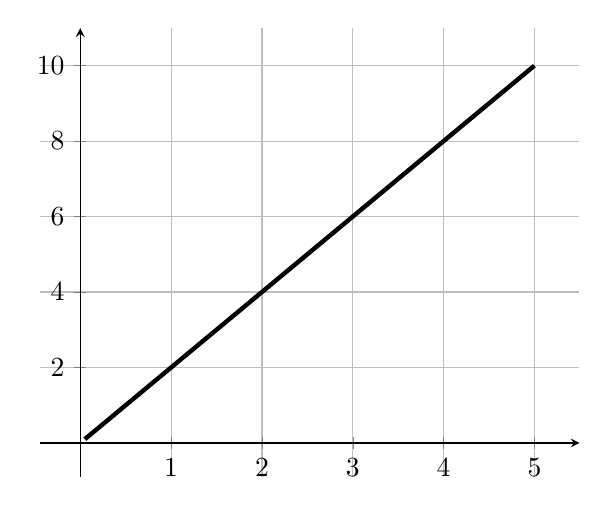
\begin{tikzpicture}
			\begin{axis}[grid=both,
				xmax=5,ymax=10,
				axis lines=middle,
				restrict x to domain=0:6,
				restrict y to domain=0:11,
				samples=100,
				enlargelimits]
				\addplot[black, ultra thick]  {2*x};
			\end{axis}
		\end{tikzpicture}
	\end{center}
	Una buona approssimazione potrebbe essere
	\begin{equation*}
		h(x)=w_1 x + w_0 = 2x
	\end{equation*}
\end{example}
\subsubsection{Univariata}
In questo esempio abbiamo 1 variabile di input $x$ e una di output $y$.
\begin{definition}[Modello]
	Un modello $h_w(x)$ è espresso come
	\begin{equation}
		out=h(x)=w_1x+w_0+noise
	\end{equation}
	dove $w_1$ e $w_0$ sono parametri liberi mentre $noise$ è una certa tolleranza.
\end{definition}
\noindent Dobbiamo quindi modificare i valori dei parametri liberi $w_1$ e $w_0$ per fare un \textbf{fitting} dei dati.\\
Una volta costruito il modello basta applicare la funzione $h(x)$ ad un determinato input $x'$.\\\\
Nonostante lo spazio delle ipotesi sia infinito (i parametri liberi sono continui), si può utilizzare il \textbf{metodo dei minimi quadrati}.
\begin{definition}[LMS]
	Dato un training set $l$ del tipo $(x_p,y_p)$, trovare un modello di regressione univariata con dei parametri liberi che minimizzi l'errore medio sui training data.
	\begin{equation*}
		Loss(h_w) = E(w) = \sum_{p=1}^{l} (y_p - h_w(x_p))^2 = \sum_{p=1}^{l} (y_p - (w_1 x_p + w_0))^2
	\end{equation*}
	Per ottenere la media è sufficiente dividere per $l$.
\end{definition}
\noindent Per risolvere questo minimo è sufficiente calcolare il gradiente e porlo uguale a $0$:
\begin{equation*}
	w_1 = \frac{\sum_{p=1}^{l} x_py_p - \frac{1}{l}\sum_{p=1}^{l} x_p\sum_{p=1}^{l} y_p}{\sum_{p=1}^{l} x^2 - \frac{1}{l}(\sum_{p=1}^{l} x_p)^2} = \frac{Cov[x,y]}{Var[x]} \quad\quad w_0=\frac{1}{l}\sum_{p=1}^{l} y_p - w_1 \sum_{p=1}^{l} x_p
\end{equation*}
In particolare, il gradiente della funzione LMS per ogni istante (possiamo quindi omettere $p$) è:
\begin{equation}
	\frac{\delta E(w)}{\delta w_0} = -2(y-h_w(x)) \quad\quad \frac{\delta E(w)}{\delta w_1} = -2(y-h_w(x))\cdot x
\end{equation}
Possiamo utilizzare un algoritmo che si basa sul concetto dell'\hyperref[alg:hill_climbing]{Hill Climbing}: da un punto scelto a caso ci spostiamo nella direzione che ci indica il gradiente:
\begin{equation}
	w_{new} = w + \eta \cdot \Delta w
\end{equation}
Dove $eta$ è il \textbf{learning rate} e $\Delta w = - \text{gradient of }E(w)$.
\begin{definition}[Delta rule]
	È una regola di correzione degli errori che cambia i parametri liberi in proporzione all'errore $target-output$:
	\begin{itemize}
		\item L'errore è $0$, non facciamo correzioni
		\item L'output è troppo alto ($y-h<0$)
		\begin{itemize}
			\item Se $\Delta w_0$ è negativo, riduciamo $w_0$
			\item Se $x>0$ e $\Delta w_1$ è negativo, riduciamo $w_1$, altrimenti lo aumentiamo
		\end{itemize}
		\item L'output è troppo basso ($y-h>0$)
	\end{itemize}
\end{definition}
\noindent Si noti che:
\begin{equation}
	\Delta w_0 = -\frac{\delta E(w)}{\delta w_0} = 2\sum_{p=1}^{l}(y_p - h_w(x_p)) \quad\quad\Delta w_1 = -\frac{\delta E(w)}{\delta w_1} = 2\sum_{p=1}^{l}(y_p - h_w(x_p)) \cdot x_p
\end{equation}
Possiamo seguire due tecniche:
\begin{itemize}
	\label{def:batch_online}
	\item \textbf{Batch algorithm}: mi muovo solo dopo aver calcolato tutti i dati ed aver fatto la sommatoria, alla fine di un'\textbf{epoca}
	\item \textbf{On-line algorithm}: ad ogni valore calcolato mi muovo, è \textit{stocastico} e di conseguenza serve un \textit{learning rate} più basso
\end{itemize}
\subsubsection{Multivariata}
Quando abbiamo $l$ pattern in input di dimensione $n$, possiamo rappresentarli in forma matriciale come segue:
\begin{table}[!h]
	\centering
	\begin{tabular}{|c|c|c|c|c|}
		\hline
		\textbf{Pattern} & $x_1$ & $x_2$ & $x_i$ & $x_n$ \\
		\hline
		Pat 1 & $x_{1,1}$ & $x_{1,2}$ & $\ldots$ & $x_{1,n}$ \\
		\hline
		$\ldots$ & & & & \\
		\hline
		Pat p & $x_{p,1}$ & $x_{p,2}$ & $x_{p,i}$ & $x_{p,n}$ \\
		\hline
		$\ldots$ & & & & \\
		\hline
	\end{tabular}
\end{table}
\\ Ogni riga rappresenta un generico pattern $\mathbf{x}$ e $x_{p,i}$ è la componente i-esima del pattern $p$.\\
Rappresentandolo quindi in termini di regressione univariata avremo
\begin{equation}
	\mathbf{w}^T\mathbf{x} + w_0 = w_0 + w_1x_1 + w_2x_2 + \ldots  + w_nx_n = w_0 + \sum_{i=1}^{n} w_i x_i
\end{equation}
\begin{note}
	È comodo includere anche la costante $x_0=1$ in modo da poter scrivere
	\begin{equation*}
		\mathbf{w}^Tx = \mathbf{x}^T w \quad\quad \mathbf{x}^T = [1, x_1, x_2, \ldots, x_n] \quad \quad \mathbf{w}^T = [w_0, w_1, w_2, \ldots, w_n]
	\end{equation*}
\end{note}
\noindent Dobbiamo trovare il vettore $w$ che minimizzi l'errore:
\begin{equation}
	E(w)=\sum_{p=1}^{l} (y_p - \mathbf{x}_p^T\mathbf{w})^2 = \lvert\lvert \mathbf{y} - \mathbf{Xw}\rvert\rvert^2
\end{equation} e possiamo ancora applicare l'Hill Climbing iterativo:
\begin{equation}
	\Delta w_i = -\frac{\delta E(\mathbf{w})}{\delta w_i} = 2\sum_{p=1}^{l}(y_p - h_\mathbf{w}(\mathbf{x}_p)) \cdot x_{p,i} = 2\sum_{p=1}^{l}(y_p - \mathbf{x}_p^T \mathbf{w}) \cdot x_{p,i}
\end{equation}
di conseguenza:
\begin{equation}
	\Delta w = - \frac{\delta E(\mathbf{w})}{\delta \mathbf{w}} = \begin{bmatrix}
		- \frac{\delta E(\mathbf{w})}{\delta w_1} \\
		- \frac{\delta E(\mathbf{w})}{\delta w_2} \\
		- \frac{\delta E(\mathbf{w})}{\delta w_i} \\
		\ldots \\
		- \frac{\delta E(\mathbf{w})}{\delta w_n}
	\end{bmatrix} = 
	\begin{bmatrix}
		\Delta w_1 \\
		\Delta w_2 \\
		\Delta w_i \\
		\ldots \\
		\Delta w_n
	\end{bmatrix}
\end{equation}
\subsubsection{Gradient descent}
Riassumendo, l'algoritmo consiste in:
\begin{enumerate}
	\item Si inizia con il vettore $\mathbf{w}_{initial}$ (piccolo) e un $\eta$ fisso $0 < \eta < 1$
	\item Si calcola $\Delta \mathbf{w} = - \text{gradient of } E(\mathbf{w}) = -\frac{\delta E(\mathbf{w})}{\delta \mathbf{w}}$
	\item Si calcola $\mathbf{w}_{new}=\mathbf{w} + \eta \cdot \Delta\mathbf{w}$
	\item Si ripete dal punto 2 finché si converge o si raggiunge un errore sufficientemente piccolo
\end{enumerate}
Anche qui per utilizzare la media è sufficiente fare $\frac{\Delta w}{l}$ e si possono utilizzare le due tecniche spiegate in \hyperref[def:batch_online]{precedenza}.

\begin{definition}[Curva di apprendimento]
	Sono curve che mostrano come l'errore decresce ad ogni iterazione del gradiente.
	\begin{center}
		\includegraphics[scale=0.3]{learning_curve.png}
	\end{center}
\end{definition}
\subsubsection{Limitazioni}
Una chiara limitazione della regressione lineare è descritta dal seguente esempio:
\begin{center}
	\includegraphics[scale=0.2]{linear_limitations.png}
\end{center}
\subsubsection{Linear Basis Expansion}
Il modello che abbiamo visto fino ad ora è lineare rispetto al vettore $\mathbf{w}$ e non rispetto a $\mathbf{x}$. Di conseguenza possiamo combinare il primo con degli input e output non lineari, sempre mantenendo la linearità del modello.
\begin{definition}[LBE]
	Dati un numero di parametri $K$ e una trasformazione generica $\phi$, una linear basis expansion è:
	\begin{equation}
		h_w(\mathbf{x}) = \sum_{k=0}^{K}w_k \phi_k(\mathbf{x})
	\end{equation}
\end{definition}
\begin{example}[LBE]
	Alcuni esempi di LBE:
	\begin{align*}
		&  \phi_j(x)=x^j \quad\quad h(\mathbf{x})=w_0+w_1x+w_2x^2+\ldots+w_Mx^M = \sum_{j=0}^{M}w_jx^j\\
		& \phi(\mathbf{x})=\phi([x_1,x_2,x_3]) \quad\quad h(\mathbf{x})=w_1x_1+w_2x_2 + w_3 \log(x_2)+w_4 \log (x_3) + w_5(x_2x_3)+w_0
	\end{align*}
\end{example}
\noindent Questa tecnica aumenta notevolmente l'espressività ma aggiunge anche due difetti principali:
\begin{itemize}
	\item Bisogna capire quali trasformazioni scegliere
	\item Bisogna tenere conto della complessità del modello (differente dalla complessità di calcolo)
\end{itemize}
\begin{example}
	\label{example:LBE}
	Con una regressione lineare al primo grado abbiamo \textbf{underfitting}, mentre con una al nono grado abbiamo \textbf{overfitting} (il modello è troppo \textit{complesso}, precisissimo sul training set ma non sul test set). La scelta migliore in questo caso sarebbe il terzo grado.
	\begin{center}
		\begin{minipage}{0.48\linewidth}
			\centering
			\includegraphics[scale=0.2]{LBE_1.png}
			\captionof{figure}{Primo grado}
		\end{minipage}
		\begin{minipage}{0.48\linewidth}
			\centering
			\includegraphics[scale=0.2]{LBE_3.png}
			\captionof{figure}{Terzo grado}
		\end{minipage}
		\includegraphics[scale=0.2]{LBE_9.png}
		\captionof{figure}{Nono grado}
	\end{center}
\end{example}

\begin{definition}[Complessità]
	Nell'ambito del ML la complessità non è il costo computazionale ma è una misura della flessibilità del modello per adattarsi correttamente ai dati.
\end{definition}
\newpage
\subsection{Regolarizzazione}
La regolarizzazione consiste nel gestire l'\textbf{overfitting} penalizzando la complessità delle funzioni mantenendo la flessibilità del modello.
\subsubsection{Ridge regression}
Questo tipo di regressione permette di ammorbidire il modello, ovvero rendendolo meno complesso, ponendo dei vincoli sulla somma della norma dei pesi $\lvert w_j \rvert$.
\begin{definition}[Loss di Tiknhonov]
	Dato un coefficiente di regolarizzazione $\lambda$, definiamo la \textit{Loss} come:
	\begin{equation}
		Loss(h_\mathbf{w})=\sum_{p=1}^{l}(y_p-h_\mathbf{w}(\mathbf{x}_p))^2 + \lambda \lvert\lvert \mathbf{w}\rvert\rvert^2 \quad\quad \lvert\lvert \mathbf{w}\rvert\rvert^2 = \sum_i w_i^2
	\end{equation}
\end{definition}
Se prima dovevo modificare il grado del polinomio per adeguare il fitting, ora ho un modo più \textbf{generale} per una qualunque trasformazione anche non polinomiale.\\
Da questa nuova formula troviamo la nuova regola di apprendimento.
\begin{equation}
	\mathbf{w}_{new} = \mathbf{w} + \eta \cdot \Delta w - 2 \lambda \mathbf{w}
\end{equation}
\begin{example}
	Partendo dai dati dell'esempio \ref{example:LBE}, se manteniamo il grado $M=9$ ma aggiungiamo la regolarizzazione otteniamo un buon fitting. È da notare però che scegliendo $\lambda$ troppo alto abbiamo un problema di \textbf{underfitting}.
	\begin{center}
		\begin{minipage}{0.48\linewidth}
			\centering
			\includegraphics[scale=0.2]{LBE_reg.png}
			\captionof{figure}{$\log\lambda=-18$}
		\end{minipage}
		\begin{minipage}{0.48\linewidth}
			\centering
			\includegraphics[scale=0.2]{LBE_reg_1.png}
			\captionof{figure}{$\log\lambda=0$}
		\end{minipage}
	\end{center}
\end{example}
\noindent È fondamentale la scelta di $\lambda$, in quanto:
\begin{itemize}
	\item Con $\lambda$ troppo piccolo, dò più peso all'errore e rischio l'\textbf{overfitting}
	\item Con $\lambda$ grande, dò meno peso all'errore e rischio l'\textbf{underfitting}
\end{itemize}
\begin{center}
	\includegraphics[scale=0.3]{LBE_lambda.png}
\end{center}

\begin{observation}[Curse of dimensionality]
	Quando aggiungiamo funzioni più complesse tramite la LBE ad un modello n-dimensionale, i dati diventano molto più sparsi e quelli necessari a supportare il risultato aumentano esponenzialmente.
\end{observation}

\subsection{Classification}

